\documentclass[12pt]{article}
\usepackage[papersize={5.5in,8.5in},top=0.4in,bottom=0.5in,left=0.4in, right=0.4in]{geometry}
% \usepackage[papersize={5.5in,8.5in},margin=0.35in,includefoot]{geometry}

\usepackage{makeidx}
\usepackage[noprint,1to1]{booklet}
% \usepackage[print,1to1]{booklet} \nofiles
\source{\magstep0}{5.5in}{8.5in}
\target{\magstep0}{11in}{8.5in}
\setpdftargetpages
\makeindex

\usepackage[T1]{fontenc}
\usepackage[utf8]{inputenc}
\usepackage{microtype}
\usepackage{titlesec}
\usepackage{ebgaramond}
\usepackage{xcolor}
\usepackage{multicol}
\usepackage{enumitem}
\usepackage{tocloft}
\usepackage{yfonts}
\usepackage{graphicx}
\usepackage[object=vectorian]{pgfornament}
\usetikzlibrary{shapes.geometric,calc}

\titleformat\section{\normalfont\Large\bfseries}{}{0em}{}
\titleformat\subsection{\normalfont\large\bfseries}{}{0em}{}

\newcommand\cmg[1]{{\color{gray}[#1]}}
\newcommand\sentspace{\spacefactor\sfcode`.{}}

\titleformat\section{\normalfont\Large\bfseries}{}{0em}{}
% \titleformat\subsection{\normalfont\itshape}{}{0em}{}
% \titleformat\paragraph[runin]{\normalfont\itshape}{}{0em}{}

% \titlecontents{subsection}[0em]{\vskip 0.5ex}{}{\itshape}{}
\renewcommand\numberline[1]{}

\def\contentsname{\empty}

\raggedright

\newcounter{ornnumb}



\begin{document}

\vspace*{\fill}
\begin{center}
  
\begin{tikzpicture}[every node/.style={inner sep=0pt}]
  \node[text height=8cm,text width=10cm,inner sep=0pt](vecbox){}; 
  \node[anchor=north west] at (vecbox.north west){\pgfornament[width=2cm]{63}};
  \node[anchor=north east] at (vecbox.north east){\pgfornament[width=2cm,symmetry=v]{63}};
  \node[anchor=south west] at (vecbox.south west){\pgfornament[width=2cm,symmetry=h]{63}};
  \node[anchor=south east] at (vecbox.south east){\pgfornament[width=2cm,symmetry=c]{63}};
  \node[anchor=north] at (vecbox.north){\pgfornament[width=6cm,symmetry=h]{46}};
  \node[anchor=south] at (vecbox.south){\pgfornament[width=6cm]{46}};
  \node[anchor=north,rotate=90] at (vecbox.west){\pgfornament[width=4cm,symmetry=h]{46}};
  \node[anchor=north,rotate=-90] at (vecbox.east){\pgfornament[width=4cm,symmetry=h]{46}};
  \node[inner sep=6pt] (text) at (vecbox.center){\Huge Christmas Carols};
  \node[anchor=south east] at (text.north){\pgfornament[width=2.9cm]{79}};
  \node[anchor=south west] at (text.north){\pgfornament[width=2.9cm,symmetry=v]{79}};
  % \node[anchor=north] at (text.south){\pgfornament[width=5cm]{60}};
  \node[anchor=north east] at (text.south){\pgfornament[width=2.9cm,symmetry=h]{78}};
  \node[anchor=north west] at (text.south){\pgfornament[width=2.9cm,symmetry=c]{78}};
  % \node[anchor=south] at (text.north){\pgfornament[width=5cm,symmetry=h]{49}};
  \end{tikzpicture} 
\end{center}

\pagenumbering{gobble}
\vfill
\begin{center}
  \begin{tikzpicture}[every node/.style={inner sep=0pt}]
  \node[text height=7cm,text width=10cm,inner sep=0pt](vecbox){}; 
  %\node[anchor=north west] at (vecbox.north west){\pgfornament[width=2cm]{63}};
  %\node[anchor=north east] at (vecbox.north east){\pgfornament[width=2cm,symmetry=v]{63}};
  %\node[anchor=south west] at (vecbox.south west){\pgfornament[width=2cm,symmetry=h]{63}};
  %\node[anchor=south east] at (vecbox.south east){\pgfornament[width=2cm,symmetry=c]{63}};
  \node[inner sep=6pt] (text) at (vecbox.center){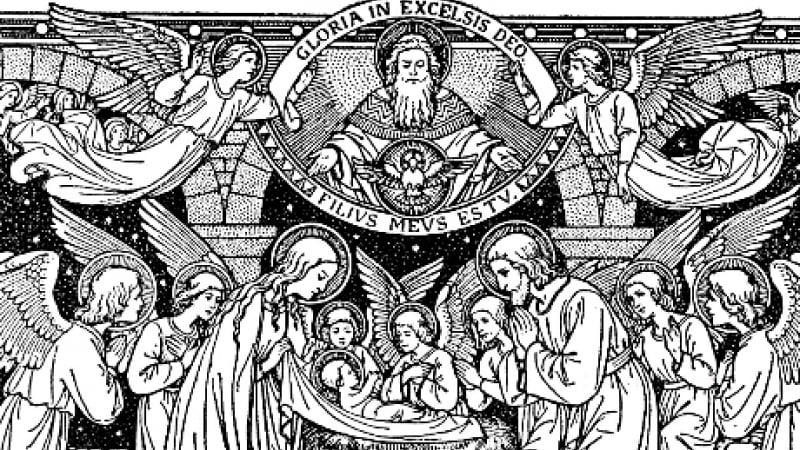
\includegraphics[width=9cm]{cover-image}};
  \node[anchor=north] at (vecbox.north){\pgfornament[width=9cm,symmetry=h]{87}};
  \node[anchor=south] at (vecbox.south){\pgfornament[width=9cm]{87}};
  \node[anchor=north,rotate=90] at (vecbox.west){\pgfornament[width=6cm,symmetry=h]{87}};
  \node[anchor=north,rotate=-90] at (vecbox.east){\pgfornament[width=6cm,symmetry=h]{87}};
  \end{tikzpicture} 
  
\end{center}

\vfill

\newpage
\vspace*{\fill}
% \hspace{-0.19in}
\makebox[\textwidth][c]{%
  \small
  \begin{minipage}{3in}
  % \begin{multicols}{2}
      \tableofcontents
  % \end{multicols}
  \end{minipage}
}
\vfill

\newpage
\pagenumbering{arabic}

\setlength\parindent{1em}
\setlength\parskip{0.8ex}

\begin{multicols}{2}
  \subsection{Adeste Fidelis}\label{adeste}
\begin{description}[nosep,leftmargin=\parindent,labelsep=0pt]
\item 1. Adeste Fideles laeti triumphantes, 
\item Veníte, veníte in Bethlehem. 
\item Natum vidéte, Regem Angelorum: 
\vspace{1.5ex}
\item (Refrain) 
\item Veníte adoremus, 
\item Veníte adoremus 
\item Veníte adoremus Dóminum 
\vspace{1.5ex}
\item 2. Deum de Deo, lumen de lúmine, 
\item gestant puellae viscera 
\item Deum verum, genitum non factum: 
\item (Refrain) 
\vspace{1.5ex}
\item 3. Cantet nunc io chorus Angelórum 
\item cantet nunc aula caelestium: 
\item Gloria in excelsis Deo: 
\item (Refrain) 
\vspace{1.5ex}
\item 4. Ergo qui natus, die hodierna 
\item Jesu, tibi sit glória 
\item Patris aeterni Verbum caro factum: 
\item (Refrain) 
\end{description}
\subsection{Angels We Have Heard on High}\label{angels_we_have_heard_on_high}
\begin{description}[nosep,leftmargin=\parindent,labelsep=0pt]
\item 1. Angels we have heard on high 
\item Sweetly singing o'er the plains, 
\item And the mountains in reply 
\item Echoing their joyous strains. 
\vspace{1.5ex}
\item (Refrain) 
\item Gloria, in excelsis Deo! 
\item Gloria, in excelsis Deo! 
\vspace{1.5ex}
\item 2. Shepherds, why this jubilee? 
\item Why your joyous strains prolong? 
\item What the gladsome tidings be 
\item Which inspire your heavenly song? 
\item (Refrain) 
\vspace{1.5ex}
\item 3. Come to Bethlehem and see 
\item Him whose birth the angels sing; 
\item Come, adore on bended knee, 
\item Christ the Lord, the newborn King. 
\item (Refrain) 
\vspace{1.5ex}
\item 4. See Him in a manger laid, 
\item Whom the choirs of angels praise; 
\item Mary, Joseph, lend your aid, 
\item While our hearts in love we raise. 
\item (Refrain) 
\end{description}
\subsection{Away in a Manger}\label{away_in}
\begin{description}[nosep,leftmargin=\parindent,labelsep=0pt]
\item 1. Away in a manger, no crib for His bed, 
\item The little Lord Jesus laid down His sweet head; 
\item The stars in the sky looked down where He lay, 
\item The little Lord Jesus, asleep in the hay. 
\vspace{1.5ex}
\item 2. The cattle are lowing, the poor Baby wakes. 
\item But little Lord Jesus, no crying He makes. 
\item I love thee, Lord Jesus, look down from the sky. 
\item And stay by the cradle till morning is nigh. 
\vspace{1.5ex}
\item 3. Be near me, Lord Jesus, I ask Thee to stay, 
\item Close by me forever, and love me, I pray! 
\item Bless all the dear children in Thy tender care 
\item And take us to heaven, to Live with Thee there. 
\end{description}
\subsection{Ding Dong Merrily on High}\label{ding_dong}
\begin{description}[nosep,leftmargin=\parindent,labelsep=0pt]
\item 1. Ding Dong! merrily on high 
\item In heav'n the bells are ringing 
\item Ding, dong! verily the sky 
\item Is riv'n with angel singing 
\item Gloria, Hosanna in excelsis 
\vspace{1.5ex}
\item 2. E'en so here below, below 
\item Let steeple bells be swungen 
\item And i-o, i-o, i-o 
\item By priest and people be sungen 
\item Gloria, Hosanna in excelsis 
\vspace{1.5ex}
\item 3. Pray ye dutifully prime 
\item Your matin chime, ye ringers 
\item May ye beautifully rime 
\item Your evetime song, ye singers 
\item Gloria, Hosanna in excelsis. 
\end{description}
\subsection{Gloucestershire Wassail}\label{wassail}
\begin{description}[nosep,leftmargin=\parindent,labelsep=0pt]
\item 1. Wassail! wassail! all over the town, 
\item Our toast it is white and our ale it is brown; 
\item Our bowl it is made of the white maple tree; 
\item With the wassailing bowl  we'll drink to thee. 
\vspace{1.5ex}
\item 2. Here's to our horse, and to his right ear, 
\item God send our master a happy new year: 
\item A happy new year as e'er he did see, 
\item With my wassailing bowl I drink to thee. 
\vspace{1.5ex}
\item 3. So here is to Cherry and to his right cheek 
\item Pray God send our master a good piece of beef 
\item And a good piece of beef that may we all see 
\item With the wassailing bowl, we'll drink to thee. 
\vspace{1.5ex}
\item 4. Here's to our mare, and to her right eye, 
\item God send our mistress a good Christmas pie; 
\item A good Christmas pie as e'er I did see, 
\item With my wassailing bowl I drink to thee. 
\vspace{1.5ex}
\item 5. So here is to Broad Mary and to her broad horn 
\item May God send our master a good crop of corn 
\item And a good crop of corn that may we all see 
\item With the wassailing bowl, we'll drink to thee. 
\vspace{1.5ex}
\item 6. And here is to Fillpail and to her left ear 
\item Pray God send our master a happy New Year 
\item And a happy New Year as e'er he did see 
\item With the wassailing bowl, we'll drink to thee. 
\vspace{1.5ex}
\item 7. Here's to our cow, and to her long tail, 
\item God send our master us never may fail 
\item Of a cup of good beer: I pray you draw near, 
\item And our jolly wassail it's then you shall hear. 
\vspace{1.5ex}
\item 8. Come butler, come fill us a bowl of the best 
\item Then we hope that your soul in heaven may rest 
\item But if you do draw us a bowl of the small 
\item Then down shall go butler, bowl and all. 
\vspace{1.5ex}
\item 9. Be here any maids? I suppose here be some; 
\item Sure they will not let young men stand on the cold stone! 
\item Sing hey O, maids! come trole back the pin, 
\item And the fairest maid in the house let us all in. 
\vspace{1.5ex}
\item 10. Then here's to the maid in the lily white smock 
\item Who tripped to the door and slipped back the lock 
\item Who tripped to the door and pulled back the pin 
\item For to let these jolly wassailers in. 
\end{description}
\subsection{God Rest Ye Merry, Gentlemen}\label{god_rest_ye}
\begin{description}[nosep,leftmargin=\parindent,labelsep=0pt]
\item 1. God rest you merry, gentlemen, 
\item Let nothing you dismay. 
\item For Jesus Christ our Savior, 
\item Was born on Christmas Day; 
\item To save us all from Satan’s power, 
\item When we were gone astray. 
\vspace{1.5ex}
\item (Chorus) 
\item O tidings of comfort and joy, 
\item Comfort and joy 
\item O tidings of comfort and joy. 
\vspace{1.5ex}
\item 2. In Bethlehem, in Jury, 
\item This blessed Babe was born, 
\item And laid within a manger, 
\item Upon this blessed morn; 
\item The which His mother Mary 
\item Did nothing take in scorn. 
\item (Chorus) 
\vspace{1.5ex}
\item 3. From God our heavenly Father, 
\item A blessed angel came. 
\item And unto certain shepherds, 
\item Brought tidings of the same, 
\item How that in Bethlehem was born, 
\item The Son of God by name: 
\item (Chorus) 
\vspace{1.5ex}
\item 4. Fear not, then said the Angel, 
\item Let nothing you affright, 
\item This day is born a Savior, 
\item Of virtue, power, and might; 
\item So frequently to vanquish all, 
\item The friends of Satan quite; 
\item (Chorus) 
\vspace{1.5ex}
\item 5. The shepherds at those tidings, 
\item Rejoiced much in mind, 
\item And left their flocks a feeding, 
\item In tempest, storm, and wind, 
\item And went to Bethlehem straightway, 
\item This blessed babe to find: 
\item (Chorus) 
\vspace{1.5ex}
\item 6. But when to Bethlehem they came, 
\item Whereas this infant lay 
\item They found him in a manger, 
\item Where oxen feed on hay; 
\item His mother Mary kneeling, 
\item Unto the Lord did pray: 
\item (Chorus) 
\vspace{1.5ex}
\item 7. With sudden joy and gladness 
\item The shepherds were beguiled, 
\item To see the Babe if Israel, 
\item Before His mother mild, 
\item O then with joy and cheerfulness 
\item Rejoice, each mother's child. 
\item (Chorus) 
\vspace{1.5ex}
\item 8. Now to the Lord sing praises, 
\item All you within this place, 
\item And with true love and brotherhood, 
\item Each other now embrace; 
\item This holy tide of Christmas, 
\item Doth bring redeeming grace. 
\item (Chorus) 
\vspace{1.5ex}
\item 9. God bless the ruler of this house, 
\item And send him long to reign, 
\item And many a merry Christmas 
\item May live to see again; 
\item Among your friends and kindred 
\item That live both far and near. 
\item (Alternate Chorus): 
\vspace{1.5ex}
\item That God send you a happy new year, 
\item Happy new year, 
\item And God send you a happy new year. 
\end{description}
\subsection{Good Christian Men, Rejoice}\label{good_christian_friends}
\begin{description}[nosep,leftmargin=\parindent,labelsep=0pt]
\item 1. Good Christian men, rejoice 
\item With heart, and soul, and voice; 
\item Give ye heed to what we say: 
\item Jesus Christ was born to-day: 
\item Ox and ass before Him bow, 
\item And He is in the manger now. 
\item Christ is born today! Christ is born today. 
\vspace{1.5ex}
\item 2. Good Christian men, rejoice, 
\item With heart, and soul, and voice; 
\item Now ye hear of endless bliss: 
\item Jesus Christ was born for this! 
\item He hath ope'd2 the heav'nly door, 
\item And man is blessed evermore.3 
\item Christ was born for this! Christ was born for this! 
\vspace{1.5ex}
\item 3. Good Christian men, rejoice 
\item With heart, and soul, and voice; 
\item Now ye need not fear the grave: 
\item Jesus Christ was born to save! 
\item Calls you one, and calls you all, 
\item To gain His everlasting hall: 
\item Christ was born to save! Christ was born to save! 
\end{description}
\subsection{Good King Wenceslas}\label{wenceslas}
\begin{description}[nosep,leftmargin=\parindent,labelsep=0pt]
\item 1. Good King Wenceslas look'd out, 
\item On the Feast of Stephen; 
\item When the snow lay round about, 
\item Deep, and crisp, and even: 
\item Brightly shone the moon that night, 
\item Though the frost was cruel, 
\item When a poor man came in sight, 
\item Gath'ring winter fuel. 
\vspace{1.5ex}
\item 2. "Hither page and stand by me, 
\item If thou know'st it, telling, 
\item Yonder peasant, who is he? 
\item Where and what his dwelling?" 
\item "Sire, he lives a good league hence. 
\item Underneath the mountain; 
\item Right against the forest fence, 
\item By Saint Agnes' fountain." 
\vspace{1.5ex}
\item 3. "Bring me flesh, and bring me wine, 
\item Bring me pine-logs hither: 
\item Thou and I will see him dine, 
\item When we bear them thither." 
\item Page and monarch forth they went, 
\item Forth they went together; 
\item Through the rude wind's wild lament, 
\item And the bitter weather. 
\vspace{1.5ex}
\item 4. "Sire, the night is darker now, 
\item And the wind blows stronger; 
\item Fails my heart, I know now how, 
\item I can go no longer." 
\item "Mark my footsteps, good my page; 
\item Tread thou in them boldly; 
\item Thou shalt find the winter's rage 
\item Freeze thy blood less coldly." 
\vspace{1.5ex}
\item 5. In his master's steps he trod, 
\item Where the snow lay dinted; 
\item Heat was in the very sod 
\item Which the Saint had printed. 
\item Therefore, Christian men, be sure, 
\item Wealth or rank possessing, 
\item Ye who now will bless the poor, 
\item Shall yourselves find blessing. 
\end{description}
\subsection{Hark! The Hearld Angels Sing}\label{hark_the_herald}
\begin{description}[nosep,leftmargin=\parindent,labelsep=0pt]
\item 1. Hark! The Herald Angels sing, 
\item "Glory to the new-born King; 
\item Peace on earth, and mercy mild, 
\item God and sinners reconciled!" 
\item Joyful, all ye nations, rise. 
\item Join the triumph of the skies. 
\item With th' Angelic Hosts proclaim, 
\item "Christ is born in Bethlehem!" 
\item Hark! the herald angels sing, 
\item "Glory to the new-born King." 
\vspace{1.5ex}
\item 2. Christ, by highest heaven adored, 
\item Christ, the everlasting lord 
\item Late in time behold Him come, 
\item Off-spring of a Virgin's womb 
\item Veiled in flesh the Godhead see, 
\item Hail, the incarnate deity 
\item Pleased as Man with men to dwell, 
\item Jesus, our Emmanuel. 
\item Hark! the herald angels sing, 
\item "Glory to the New-born king!" 
\vspace{1.5ex}
\item 3. Hail the heav'n-born Prince of Peace, 
\item Hail, the Sun of Righteousness 
\item Light and life to all He brings, 
\item Risen with healing in His Wings. 
\item Now He lays His Glory by, 
\item Born that man no more may die 
\item Born to raise the sons of earth, 
\item Born to give them second birth. 
\item Hark! the herald angels sing, 
\item "Glory to the New-born king!" 
\vspace{1.5ex}
\item 4. Come, Desire of nations come, 
\item Fix in us Thy humble home; 
\item Oh, to all Thyself impart, 
\item Formed in each believing heart! 
\item Hark! the herald angels sing, 
\item "Glory to the new-born king; 
\item Peace on earth and mercy mild, 
\item God and sinners reconciled!" 
\item Hark! the herald angels sing, 
\item "Glory to the New-born king!" 
\vspace{1.5ex}
\item 5. Adam's likeness, Lord, efface, 
\item Stamp Thine image in its place: 
\item Second Adam from above, 
\item Reinstate us in Thy love. 
\item Let us Thee, though lost, regain, 
\item Thee, the Life, the inner man: 
\item O, to all Thyself impart, 
\item Formed in each believing heart. 
\item Hark! the herald angels sing, 
\item "Glory to the New-born king!" 
\end{description}
\subsection{I Saw Three Ships}\label{i_saw_three_ships}
\begin{description}[nosep,leftmargin=\parindent,labelsep=0pt]
\item 1. I saw three ships come sailing in, 
\item On Christmas day, on Christmas day, 
\item I saw three ships come sailing in, 
\item On Christmas day in the morning. 
\vspace{1.5ex}
\item 2. And what was in those ships all three? 
\item On Christmas day... 
\item And what was in those ships all three? 
\item On Christmas day... 
\vspace{1.5ex}
\item 3. Our Saviour Christ and his lady ... 
\item Our Saviour Christ and his lady, ... 
\vspace{1.5ex}
\item 4. Pray whither sailed those ships all three? ... 
\item Pray whither sailed those ships all three? ... 
\vspace{1.5ex}
\item 5. Oh, they sailed into Bethlehem, ... 
\item Oh, they sailed into Bethlehem, ... 
\vspace{1.5ex}
\item 6. And all the bells on earth shall ring, ... 
\item And all the bells on earth shall ring, ... 
\vspace{1.5ex}
\item 7. And all the Angels in Heaven shall sing, ... 
\item And all the Angels in Heaven shall sing, ... 
\vspace{1.5ex}
\item 8. And all the souls on earth shall sing, ... 
\item And all the souls on earth shall sing, ... 
\vspace{1.5ex}
\item 9. Then let us all rejoice, amain, ... 
\item Then let us all rejoice, amain, ... 
\end{description}
\subsection{It Came Upon the Midnight Clear}\label{midnight}
\begin{description}[nosep,leftmargin=\parindent,labelsep=0pt]
\item 1. It came upon the midnight clear, 
\item That glorious song of old, 
\item From angels bending near the earth 
\item To touch their harps of gold; 
\item "Peace on the earth, good will to men 
\item From heaven’s all-gracious King" – 
\item The world in solemn stillness lay 
\item To hear the angels sing. 
\vspace{1.5ex}
\item 2. Still through the cloven skies they come 
\item With peaceful wings unfurled, 
\item And still their heavenly music floats 
\item O'er all the weary world; 
\item Above its sad and lowly plains 
\item They bend on hovering wing, 
\item And ever o'er its Babel-sounds 
\item The blessed angels sing. 
\vspace{1.5ex}
\item 3. But with the woes of sin and strife 
\item The world has suffered long; 
\item Beneath the angel-strain have rolled 
\item Two thousand years of wrong; 
\item And man, at war with man, hears not 
\item The love song which they bring; – 
\item O hush the noise, ye men of strife, 
\item And hear the angels sing! 
\vspace{1.5ex}
\item 4. And ye, beneath life's crushing load, 
\item Whose forms are bending low, 
\item Who toil along the climbing way 
\item With painful steps and slow, 
\item Look now! for glad and golden hours 
\item Come swiftly on the wing; – 
\item Oh, rest beside the weary road 
\item And hear the angels sing! 
\vspace{1.5ex}
\item 5. For lo! the days are hastening on 
\item By prophet bards foretold, 
\item When, with the ever circling years 
\item Shall come the age of gold; 
\item When Peace shall over all the earth, 
\item Its ancient splendors fling, 
\item And the whole world give back the song, 
\item Which now the angels sing. 
\end{description}
\subsection{Joy to the World}\label{joy_to}
\begin{description}[nosep,leftmargin=\parindent,labelsep=0pt]
\item 1. Joy to the world! The Lord is come. 
\item Let earth receive her King; 
\item Let every heart prepare Him room; 
\item And heav’n and nature sing, 
\item And heav’n and nature sing. 
\item And heav’n and heav’n and nature sing. 
\vspace{1.5ex}
\item 2. Joy to the world, the Savior reigns 
\item Let men their songs employ. 
\item While fields and floods, rocks, hills, and plains 
\item Repeat the sounding joy, 
\item Repeat the sounding joy 
\item Repeat, repeat the sounding joy 
\vspace{1.5ex}
\item 3. No more let sin and sorrows grow, 
\item Nor thorns infest the ground; 
\item He comes to make His blessings flow 
\item Far as the curse is found, 
\item Far as the curse is found, 
\item Far as, far as the curse is found. 
\vspace{1.5ex}
\item 4. He rules the world with truth and grace, 
\item And makes the nations prove 
\item The glories of His righteousness. 
\item And wonders of His love, 
\item And wonders of His love, 
\item And wonders, wonders of His love. 
\end{description}
\subsection{O Come, All Ye Faithful}\label{ye_faithful}
\begin{description}[nosep,leftmargin=\parindent,labelsep=0pt]
\item 1. O come, all ye faithful, Joyful and triumphant, 
\item O Come ye, O come ye, to Bethlehem. 
\item Come and behold Him, Born the King of angels; 
\vspace{1.5ex}
\item (Refrain) 
\item O come, let us adore Him, 
\item O come, let us adore Him, 
\item O come, let us adore Him, 
\item Christ the Lord. 
\vspace{1.5ex}
\item 2. God of God, Light of Light, 
\item Lo! he abhors not the Virgin’s womb; 
\item Very God, Be-gotten not created. 
\item (Refrain) 
\vspace{1.5ex}
\item 3. Sing, choirs of angels, Sing in exultation; 
\item Sing, all ye citizens of heaven above! 
\item Glory to God, In the highest; 
\item (Refrain) 
\vspace{1.5ex}
\item 4. Yea, Lord, we greet Thee, Born this happy morning; 
\item Jesu, to Thee be glory given; 
\item Word of the Father, Now in flesh appearing. 
\item (Refrain) 
\vspace{1.5ex}
\item 5. See how the shepherds, Summoned to His cradle, 
\item Leaving their flocks, draw nigh to gaze; 
\item We too will thither Bend our hearts' oblations 
\item (Refrain) 
\end{description}
\subsection{O Holy Night}\label{o_holy_night}
\begin{description}[nosep,leftmargin=\parindent,labelsep=0pt]
\item 1. O holy night, the stars are brightly shining, 
\item It is the night of the dear Saviour’s birth; 
\item Long lay the world in sin and error pining, 
\item 'Till he appeared and the soul felt its worth. 
\item A thrill of hope the weary world rejoices, 
\item For yonder breaks a new and glorious morn; 
\vspace{1.5ex}
\item Fall on your knees, Oh hear the angel voices! 
\item O night divine! O night when Christ was born. 
\item O night, O holy night, O night divine. 
\vspace{1.5ex}
\item 2. Led by the light of Faith serenely beaming; 
\item With glowing hearts by his cradle we stand: 
\item So, led by light of a star sweetly gleaming, 
\item Here come the wise men from Orient land, 
\item The King of Kings lay thus in lowly manger, 
\item In all our trials born to be our friend; 
\vspace{1.5ex}
\item He knows our need, To our weakness no stranger! 
\item Behold your King! Before Him lowly bend! 
\item Behold your King! your King! before him bend! 
\vspace{1.5ex}
\item 3. Truly He taught us to love one another; 
\item His law is Love and His gospel is Peace; 
\item Chains shall he break, for the slave is our brother, 
\item And in his name all oppression shall cease, 
\item Sweet hymns of joy in grateful Chorus raise we; 
\item Let all within us praise his Holy name! 
\vspace{1.5ex}
\item Christ is the Lord, then ever! ever praise we! 
\item His pow'r and glory, evermore proclaim! 
\item His pow'r and glory, evermore proclaim! 
\end{description}
\subsection{O Little Town of Bethlehem}\label{o_little_town}
\begin{description}[nosep,leftmargin=\parindent,labelsep=0pt]
\item 1. O little town of Bethlehem 
\item How still we see thee lie 
\item Above thy deep and dreamless sleep 
\item The silent stars go by 
\item Yet in thy dark streets shineth 
\item The everlasting Light 
\item The hopes and fears of all the years 
\item Are met in thee tonight 
\vspace{1.5ex}
\item 2. For Christ is born of Mary 
\item And gather’d all above 
\item While mortals sleep, the angels keep 
\item Their watch of wondering love 
\item O morning stars together 
\item Proclaim the holy birth 
\item And praises sing to God the King 
\item And Peace to men on earth 
\vspace{1.5ex}
\item 3. How silently, how silently 
\item The wondrous gift is given! 
\item So God imparts to human hearts 
\item The blessings of His heav’n. 
\item No ear may hear his His coming, 
\item But in this world of sin, 
\item Where meek souls will receive him still, 
\item The dear Christ enters in. 
\vspace{1.5ex}
\item 4. O holy Child of Bethlehem 
\item Descend to us, we pray 
\item Cast out our sin and enter in 
\item Be born to us today 
\item We hear the Christmas angels 
\item The great glad tidings tell 
\item O come to us, abide with us 
\item Our Lord Emmanuel 
\end{description}
\subsection{Silent Night, Holy Night}\label{silent_night}
\begin{description}[nosep,leftmargin=\parindent,labelsep=0pt]
\item 1. Silent night! Holy night! 
\item All is calm, all is bright, 
\item Round yon Virgin Mother and Child! 
\item Holy Infant, so tender and mild, 
\item Sleep in heavenly peace! 
\item Sleep in heavenly peace! 
\vspace{1.5ex}
\item 2. Silent night! Holy night! 
\item Shepherds quake at the sight! 
\item Glories stream from Heaven afar, 
\item Heavenly Hosts sing Alleluia! 
\item Christ, the Saviour, is born! 
\item Christ, the Saviour, is born! 
\vspace{1.5ex}
\item 3. Silent night! Holy night! 
\item Son of God, love’s pure light 
\item Radiant beams from Thy Holy Face 
\item With the dawn of redeeming grace, 
\item Jesus, Lord, at Thy Birth! 
\item Jesus, Lord, at Thy Birth! 
\vspace{1.5ex}
\item 4. Silent Night, Holy Night 
\item Here at last, healing light 
\item From the heavenly kingdom sent, 
\item Abundant grace for our intent. 
\item Jesus, salvation for all. 
\item Jesus, salvation for all. 
\vspace{1.5ex}
\item 5. Silent Night! Holy Night" 
\item Sleeps the world in peace tonight. 
\item God sends his Son to earth below 
\item A Child from whom all blessings flow 
\item Jesus, embraces mankind. 
\item Jesus, embraces mankind. 
\vspace{1.5ex}
\item 6. Silent Night, Holy Night 
\item Mindful of mankind's plight 
\item The Lord in Heav'n on high decreed 
\item From earthly woes we would be freed 
\item Jesus, God's promise for peace. 
\item Jesus, God's promise for peace. 
\end{description}
\subsection{The Boar's Head Carol}\label{boars_head}
\begin{description}[nosep,leftmargin=\parindent,labelsep=0pt]
\item (Refrain) 
\item Caput apri defero 
\item Reddens laudes Domino 
\vspace{1.5ex}
\item 1. The boar’s head in hand bring I, 
\item Bedeck'd with bays and rosemary. 
\item I pray you, my masters, be merry 
\item Quot estis in convivio 
\item (Refrain) 
\vspace{1.5ex}
\item 2. The boar's head, as I understand, 
\item Is the rarest dish in all this land, 
\item Which thus bedeck'd with a gay garland 
\item Let us servire cantico. 
\item (Refrain) 
\vspace{1.5ex}
\item 3. Our steward hath provided this 
\item In honor of the King of Bliss; 
\item Which, on this day to be served is 
\item In Reginensi atrio. 
\item (Refrain) 
\end{description}
\subsection{The First Noel}\label{the_first_noel}
\begin{description}[nosep,leftmargin=\parindent,labelsep=0pt]
\item 1. The first Nowel that the Angel did say, 
\item Was to certain poor Shepherds in fields as they lay, 
\item In fields as they lay a-keeping their sheep, 
\item On a cold winter's night that was freezing so deep. 
\vspace{1.5ex}
\item (Chorus) 
\item Nowel, Nowel, Nowel, Nowel, 
\item Born is the King of Israel. 
\vspace{1.5ex}
\item 2. They looked up above, to the East where a Star 
\item That beyond them shone out in the Heavens from afar, 
\item And which to the earth did send down a great light, 
\item And so it continued by day and by night. 
\item (Chorus) 
\vspace{1.5ex}
\item 3. And then by the light of that bright guiding Star, 
\item There came three Wise Men from a country afar; 
\item To seek for a King, it was their intent, 
\item And to follow the Star wherever it went. 
\item (Chorus) 
\vspace{1.5ex}
\item 4. The Star went before them unto the North West, 
\item And seemed o'er the City of Bethlehem to rest, 
\item And there did remain by night and by day, 
\item Right over the place where Jesus Christ lay. 
\item (Chorus) 
\vspace{1.5ex}
\item 5. Then entered they all, and those Wise Men three 
\item Most reverently worshiped with low bended knee; 
\item And offered to Christ in His Sacred Presence, 
\item Gifts of Gold, and of Myrrh, and of sweet Frankincense. 
\item (Chorus) 
\vspace{1.5ex}
\item 6. And now Christians all, with most gladsome accord, 
\item Sing praises, sing praises to Jesus our Lord, 
\item That made both the Heaven, and the Earth out of nought, 
\item And with His Own Blood our Redemption hath wrought. 
\item (Chorus) 
\end{description}
\subsection{We Three Kings}\label{we_three_kings}
\begin{description}[nosep,leftmargin=\parindent,labelsep=0pt]
\item 1. We three kings of Orient are 
\item Bearing gifts, we traverse afar. 
\item Field and fountain, moor and mountain, 
\item Following yonder star. 
\vspace{1.5ex}
\item (Chorus) 
\item O Star of Wonder, Star of Night, 
\item Star with Royal Beauty bright, 
\item Westward leading, Still proceeding, 
\item Guide us to Thy perfect Light. 
\vspace{1.5ex}
\item 2. Born a King on Bethlehem plain, 
\item Gold I bring to crown Him again, 
\item King forever, 
\item Ceasing never 
\item Over us all to reign. 
\item (Chorus) 
\vspace{1.5ex}
\item 3. Frankincense to offer have I; 
\item Incense owns a Deity nigh: 
\item Prayer and praising 
\item All men raising, 
\item Worship Him God on high. 
\item (Chorus) 
\vspace{1.5ex}
\item 4. Myrrh is mine; it’s bitter perfume; 
\item Breathes a life of gathering gloom: — 
\item Sorrowing, sighing, 
\item Bleeding, dying, 
\item Sealed in the stone-cold tomb. 
\item (Chorus) 
\vspace{1.5ex}
\item 5. Glorious now behold Him arise, 
\item King and God and sacrifice. 
\item Heav'n sings 
\item Halleluia; 
\item Hallelujah the earth replies. 
\item (Chorus) 
\end{description}
\subsection{We Wish You a Merry Christmas}\label{we_wish}
\begin{description}[nosep,leftmargin=\parindent,labelsep=0pt]
\item 1. We wish you a Merry Christmas; 
\item We wish you a Merry Christmas; 
\item We wish you a Merry Christmas and a Happy New Year. 
\vspace{1.5ex}
\item (Refrain) 
\item Good tidings we bring to you and your kin; 
\item Good tidings for Christmas and a Happy New Year. 
\vspace{1.5ex}
\item 2. Oh, bring us a figgy pudding; (3x) 
\item ... and a cup of good cheer. 
\item (Refrain) 
\vspace{1.5ex}
\item 3. We won't go until we get some; (3x) 
\item ... so bring some right here. 
\item (Refrain) 
\vspace{1.5ex}
\item 4. We wish you a Merry Christmas; (3x) 
\item ... and a Happy New Year. 
\item (Refrain) 
\end{description}
\subsection{What Child Is This?}\label{what_child}
\begin{description}[nosep,leftmargin=\parindent,labelsep=0pt]
\item 1. What Child is this who, laid to rest 
\item On Mary's lap is sleeping? 
\item Whom Angels greet with anthems sweet, 
\item While shepherds watch are keeping? 
\vspace{1.5ex}
\item This, this is Christ the King, 
\item Whom shepherds guard and Angels sing; 
\item Haste, haste, to bring Him laud, 
\item The Babe, the Son of Mary. 
\vspace{1.5ex}
\item 2. Why lies He in such mean estate, 
\item Where ox and ass are feeding? 
\item Good Christians, fear, for sinners here 
\item The silent Word is pleading. 
\vspace{1.5ex}
\item Nails, spear shall pierce Him through, 
\item The cross be borne for me, for you. 
\item Hail, hail the Word made flesh, 
\item The Babe, the Son of Mary. 
\vspace{1.5ex}
\item 3. So bring Him incense, gold and myrrh, 
\item Come peasant, king to own Him; 
\item The King of kings salvation brings, 
\item Let loving hearts enthrone Him. 
\vspace{1.5ex}
\item Raise, raise a song on high, 
\item The Virgin sings her lullaby. 
\item Joy, joy for Christ is born, 
\item The Babe, the Son of Mary. 
\end{description}


\end{multicols}

% \vspace*{\fill}
% \begin{center}
%   \begin{tikzpicture}[every node/.style={inner sep=0pt}]
%   \node[text height=2cm,text width=\textwidth,inner sep=0pt](vecbox){}; 
%   % \node[inner sep=6pt] (text) at (vecbox.center){\Huge\frakfamily Christmas Carols};
%   % \node[anchor=north,rotate=0] at (text.south){\pgfornament[width=5cm]{49}};
%   \node[anchor=north east,rotate=20] at (vecbox.center) {\pgfornament[symmetry=h,width=2.5cm]{77}};
%   \node[anchor=north west,rotate=-20] at (vecbox.center) {\pgfornament[symmetry=c,width=2.5cm]{77}};
%   \node[anchor=south west,shift={(0cm,-0.40cm)},rotate=20] at (vecbox.center) {\pgfornament[symmetry=v,width=2.5cm]{77}};
%   \node[anchor=south east,shift={(0cm,-0.40cm)},rotate=-20] at (vecbox.center) {\pgfornament[width=2.5cm]{77}};
%   %\node[anchor=south] at (text.north){\pgfornament[width=5cm,symmetry=h]{49}};
%   \end{tikzpicture} 
% \end{center}
% \vfill

\newpage
\vspace*{\fill}
\begin{center}
  \pgfornament[height=0.5in]{57}
  \vfill
  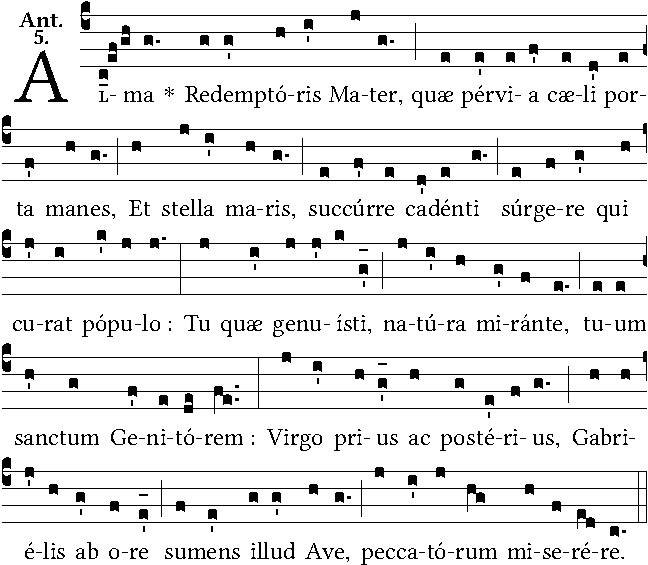
\includegraphics[width=0.9\textwidth]{alma-redemptoris}
  \vfill
  \pgfornament[symmetry=v,height=0.5in]{57}
\end{center}
\vspace*{\fill}

\newpage
\pagenumbering{gobble}
\vspace*{\fill}
\begin{center}
  \pgfornament[width=0.9\textwidth]{45}
  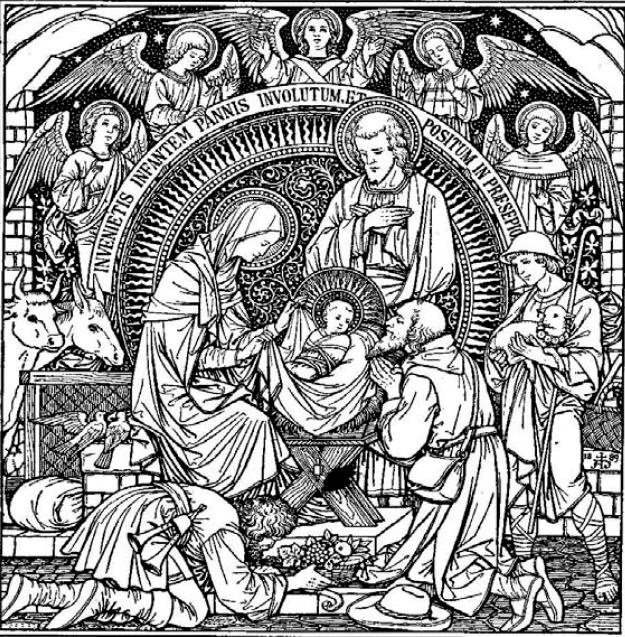
\includegraphics[width=0.9\textwidth]{back-cover}
  \pgfornament[symmetry=h,width=0.9\textwidth]{45}
\end{center}
\vspace*{\fill}

% \newpage \noindent\loop
% \ifnum\value{ornnumb}<89
% \stepcounter{ornnumb}%
% ornament~\theornnumb: \pgfornament[width=1.5cm]{\theornnumb}\\[1ex]
% \repeat

% \newpage
% \vspace*{\fill}
% \begin{center}
%   \Huge\frakfamily Merry Christmas!
% \end{center}
% \vspace*{\fill}

\end{document}
